\subsection{Software de dise\~no}

\noindent
\justify

Para la ejecuci\'on de la metodolog\'ia mostrada en la Figura \ref{metodologia}, se desarroll\'o un software de dise\~no con herramientas de \textit{c\'odigo abierto}. El software se compone, principalmente, de dos partes: \textit{Frontend} (interfaz de usuario), desarrollada en Jupyter y ParaView, y \textit{Backend} (l\'ogica detr\'as del software), desarrollada en Python, C++ y gmsh. Anexo a este trabajo se encuentran los diferentes componentes desarrollados del software; dando evidencia de la calidad de resultados obtenidos a trav\'es de este.

\subsubsection{Frontend}

\noindent
\justify

La interfaz gr\'afica se desarroll\'o en \textit{Jupyter}. El proyecto Jupyter existe para facilitar el desarrollo de software libre; trat\'andose de un servicio de computaci\'on interactiva que funciona con diferentes lenguajes de programaci\'on, entre ellos: Python y C++. Un ejemplo que permite visualizar el alcance de esta herramienta se puede apreciar en la Figura \ref{jupyter}; en d\'onde se observa la escritura de algoritmos de programaci\'on, evaluaci\'on de la interactividad del algoritmo y documentaci\'on del mismo: todo en una sola pantalla. Jupyter es un acr\'onimo de los lenguajes: \textit{Julia, Python} y \textit{R}.

\begin{figure}[h!]
	\centering
	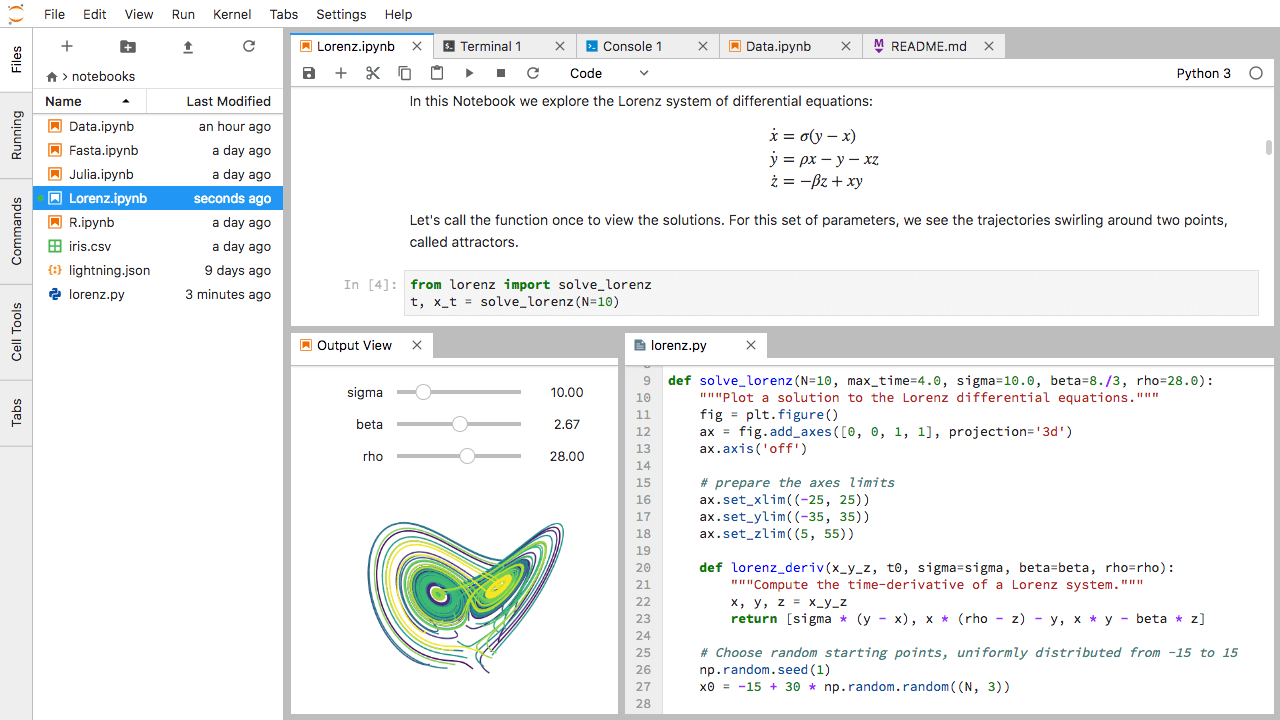
\includegraphics[width=\textwidth]{Images/jupyterlab.png}
	\caption{Interfaz gr\'afica de ejemplo desarrollada con Jupyter. Fuente: https://jupyterlab.readthedocs.io/en/latest/}
	\label{jupyter}
\end{figure}

\noindent
\justify

``Jupyter es una aplicaci\'on web de c\'odigo abierto que permite la creaci\'on y compartibilidad de diferentes documentos, encontr\'andose en ellos: c\'odigo \textit{en vivo}, ecuaciones y visualizaci\'on de texto explicativo. Entre sus usos se encuentran: limpieza y transformaci\'on de datos, simulaciones num\'ericas, modelado estad\'istico y aprendizaje autom\'atico, entre muchos otros." Descripci\'on oficial del proyecto Jupyter.

\noindent
\justify

Parte del Frontend desarrollado para brindar interactividad de usuario se puede apreciar en la Figura \ref{interfaz}.

\begin{figure}[h!]
	\centering
	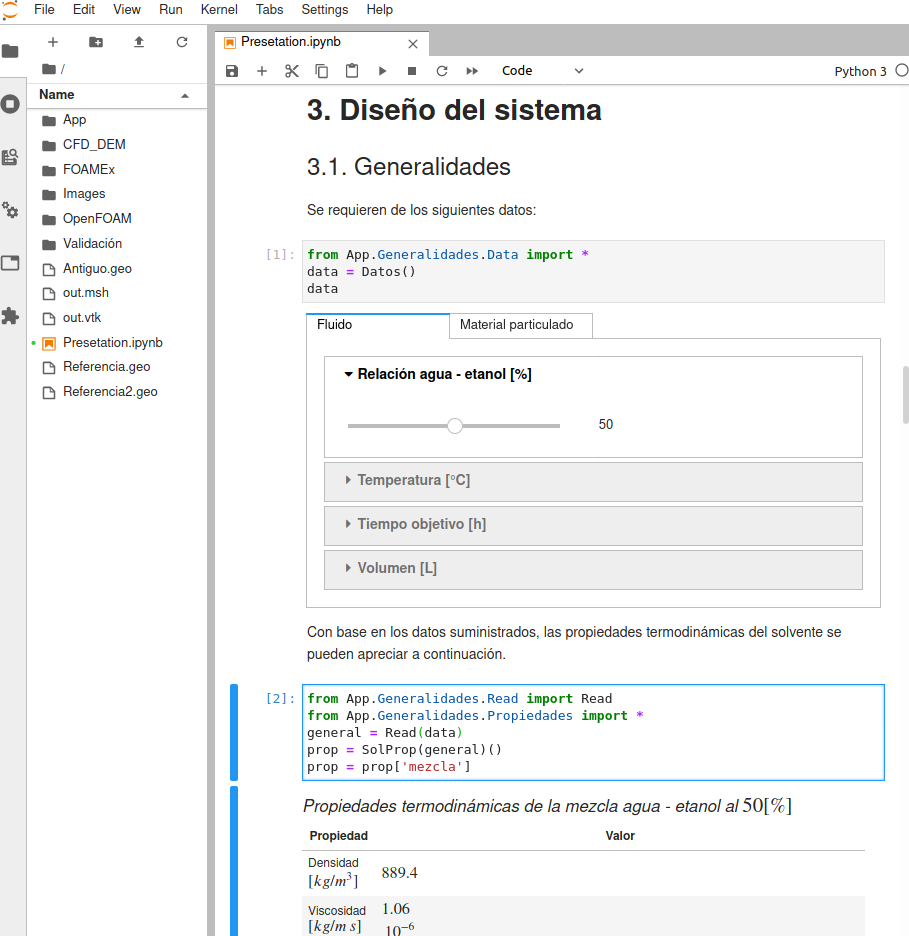
\includegraphics[width=\textwidth]{Images/interfaz.png}
	\caption{Parte de la interfaz gr\'afica desarrollada para la automatizaci\'on del modelo CFD-DEM.}
	\label{interfaz}
\end{figure}

\noindent
\justify


Jupyter permite la interactividad a trav\'es de diferentes lenguajes de Frontend; entre ellos: HTML, CSS y JavaScript. Para la escritura de textos, adopta lenguajes como Markdown y \LaTeX. Adem\'as, cuenta con diferentes librer\'ias internas para el desarrollo de contenidos interactivos, de las que se destacan: \texttt{ipywidgets}, \texttt{IPython.display} y \texttt{Plotly}. 

\begin{figure}[h!]
	\centering
	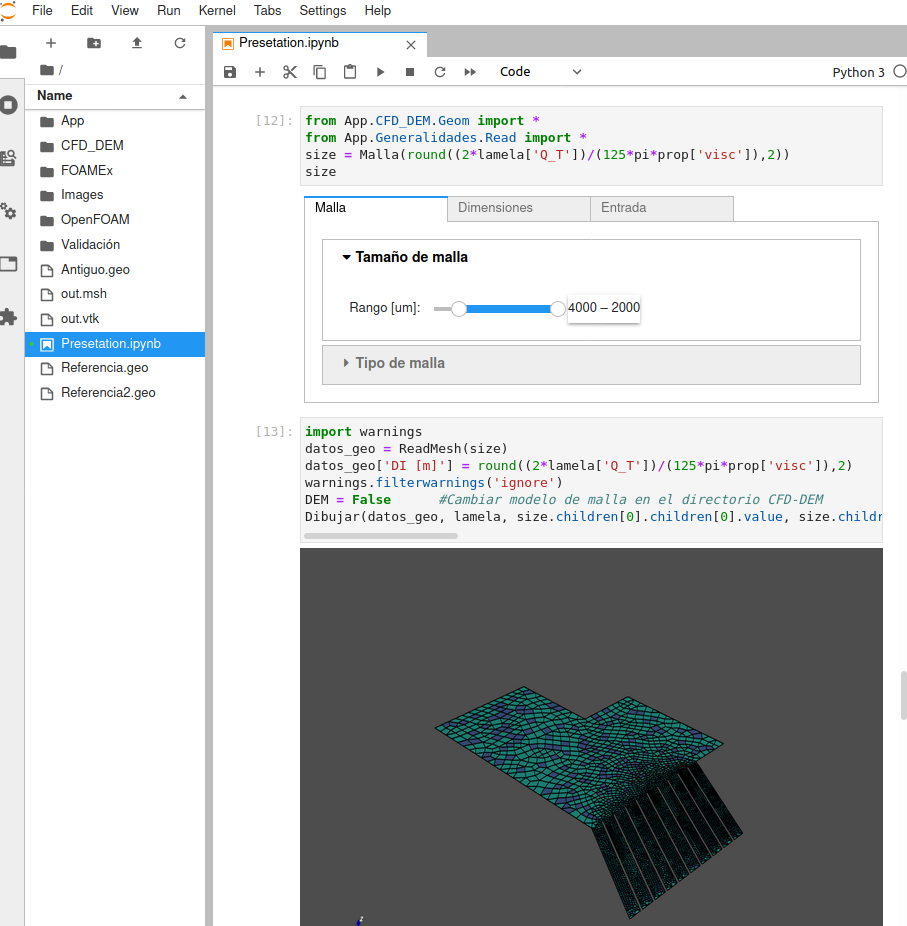
\includegraphics[width=\textwidth]{Images/interfaz2.png}
	\caption{Secci\'on de mallado autom\'atico del software desarrollado mediante \texttt{gmsh}.}
	\label{mallado:gmsh}
\end{figure}

\noindent
\justify

En la Figura \ref{mallado:gmsh} se puede apreciar la interfaz gr\'afica referente al mallado autom\'atico de la geometr\'ia, desarrollado en el lenguaje \texttt{gmsh}; en d\'onde el usuario puede definir el rango de tama\~no de malla, tipo de los elementos (rectangular o triangular) y las dimensiones de la geometr\'ia.

\newpage

\subsubsection{Backend}

\noindent
\justify

Detr\'as de la funcionalidad del software se encuentra el \'arbol de directorios mostrado en la Figura \ref{particion}.

\begin{figure}[h!]
\centering
\begin{forest}
  pic dir tree,
  where level=0{}{% folder icons by default; override using file for file icons
    directory,
  },
  [CFD-DEM Software
    [App
      [{CFD\_DEM}
        [CF.py, file
        ]
        [CFD.py, file
        ]
        [CFDEM.py, file
        ]
        [Geom.py, file
        ]        
        [Malla.py, file
        ]
      ]
      [Generalidades
        [Lamelas.py, file
        ]
        [Propiedades.py, file
        ]
        [Read.py, file
        ]
      ]
      [Sedimentaci\'on
        [Inicial.py, file
        ]      
        [ParOper.py, file
        ]
        [Resultados.py, file
        ]
      ]
    ]
    [{CFD\_DEM}
    ]
    [OpenFOAM
    ]
    [Validaci\'on
    ]
    [Presentation.ipynb, file
    ]
  ]
\end{forest}
\caption{\'Arbol de directorios.}
\label{particion}
\end{figure}

\newpage

\noindent
\justify

El software resuelve, b\'asicamente, tres problemas:

\begin{itemize}
	\item Dise\~no funcional del panel de lamelas desde un enfoque te\'orico.
	\item An\'alisis del comportamiento, a trav\'es de OpenFOAM, de la din\'amica de fluidos del panel de lamelas.
	\item Simulaci\'on CFD-DEM que permite predecir la interacci\'on fluido - part\'icula a distintas condiciones de flujo.
\end{itemize}

\newpage

\paragraph{Dise\~no funcional te\'orico}

\noindent
\justify

El dise\~no funcional busca defnir una geometr\'ia inicial del panel de lamelas, para el an\'alisis consecuente mediante los m\'etodos num\'ericos de \textit{vol\'umenes finitos} y \textit{elementos discretos}, a trav\'es de metodolog\'ias te\'oricas y experimentales (cap\'itulo \ref{teorico:sed}).

\noindent
\justify

La l\'ogica desarrollada comprende los siguientes pasos:

\begin{enumerate}
	\item Definici\'on, por parte del usuario, de las propiedades del solvente (entre ellas: proporci\'on de la mezcla hidroetan\'olica) y del material particulado.
	\item C\'alculo de las propiedades termodin\'amicas del fluido.
	\item Definici\'on de la geometr\'ia del panel de lamelas.
	\item C\'alculo de las diferentes propiedades del solvente: caudal, velocidad del fluido y de la sedimentaci\'on y el n\'umero de Reynolds, por mencionar algunos.
\end{enumerate}

\noindent
\justify

Los algoritmos que emplean esta l\'ogica se encuentran ubicados en las direcciones \texttt{App/Sedimentaci\'on} y \texttt{App/Generalidades}, como se aprecia en la Figura \ref{particion}.

\paragraph{Simulaciones num\'ericas} \label{imp:CFD}

\noindent
\justify

El modelo CFD permite conocer el comportamiento del solvente dentro del volumen de control para contrastarlo con el modelo CFD-DEM. Comprende los siguientes pasos:

\begin{enumerate}
	\item Definici\'on de la geometr\'ia.
	\item Mallado de la geometr\'ia.
	\item Definici\'on de las condiciones de frontera.
	\item Desarrollo de la simulaci\'on.
	\item Postprocesamiento y presentaci\'on de resultados.
\end{enumerate}

\noindent
\justify

Los algoritmos desarrollados para el desarrollo de este modelo se encuentran ubicados en la direcci\'on \texttt{App/{CFD\_DEM}}:

\begin{itemize}
	\item \texttt{Geom.py} permite establecer la geometr\'ia del problema de acuerdo a los par\'ametros definidos por el usuario.
	\item \texttt{Malla.py} define el mallado de la geometr\'ia, ejecutando el lenguaje \textit{gmsh}.
	\item \texttt{CF.py} define las condiciones de frontera.
	\item \texttt{CFD.py} se encarga de ejecutar la simulaci\'on num\'erica a trav\'es de OpenFOAM.
\end{itemize}

\noindent
\justify

El modelo CFD-DEM predice las interacciones fluido-part\'icula del sistema de sedimentaci\'on. Emplea la misma l\'ogica descrita en la secci\'on \ref{imp:CFD}. La \'unica diferencia radica en la ejecuci\'on del algoritmo descrito en \texttt{CFD.py}; en su lugar, ejecuta el de \texttt{CFDEM.py} que contiene la metodolog\'ia de desarrollo de la simulaci\'on CFD-DEM basada en el m\'etodo Euler - Lagrange.

